\section{开发workflow}

\subsection{git workflow}
\par 方便网开发的workflow
\begin{figure}[H]
	\centering
	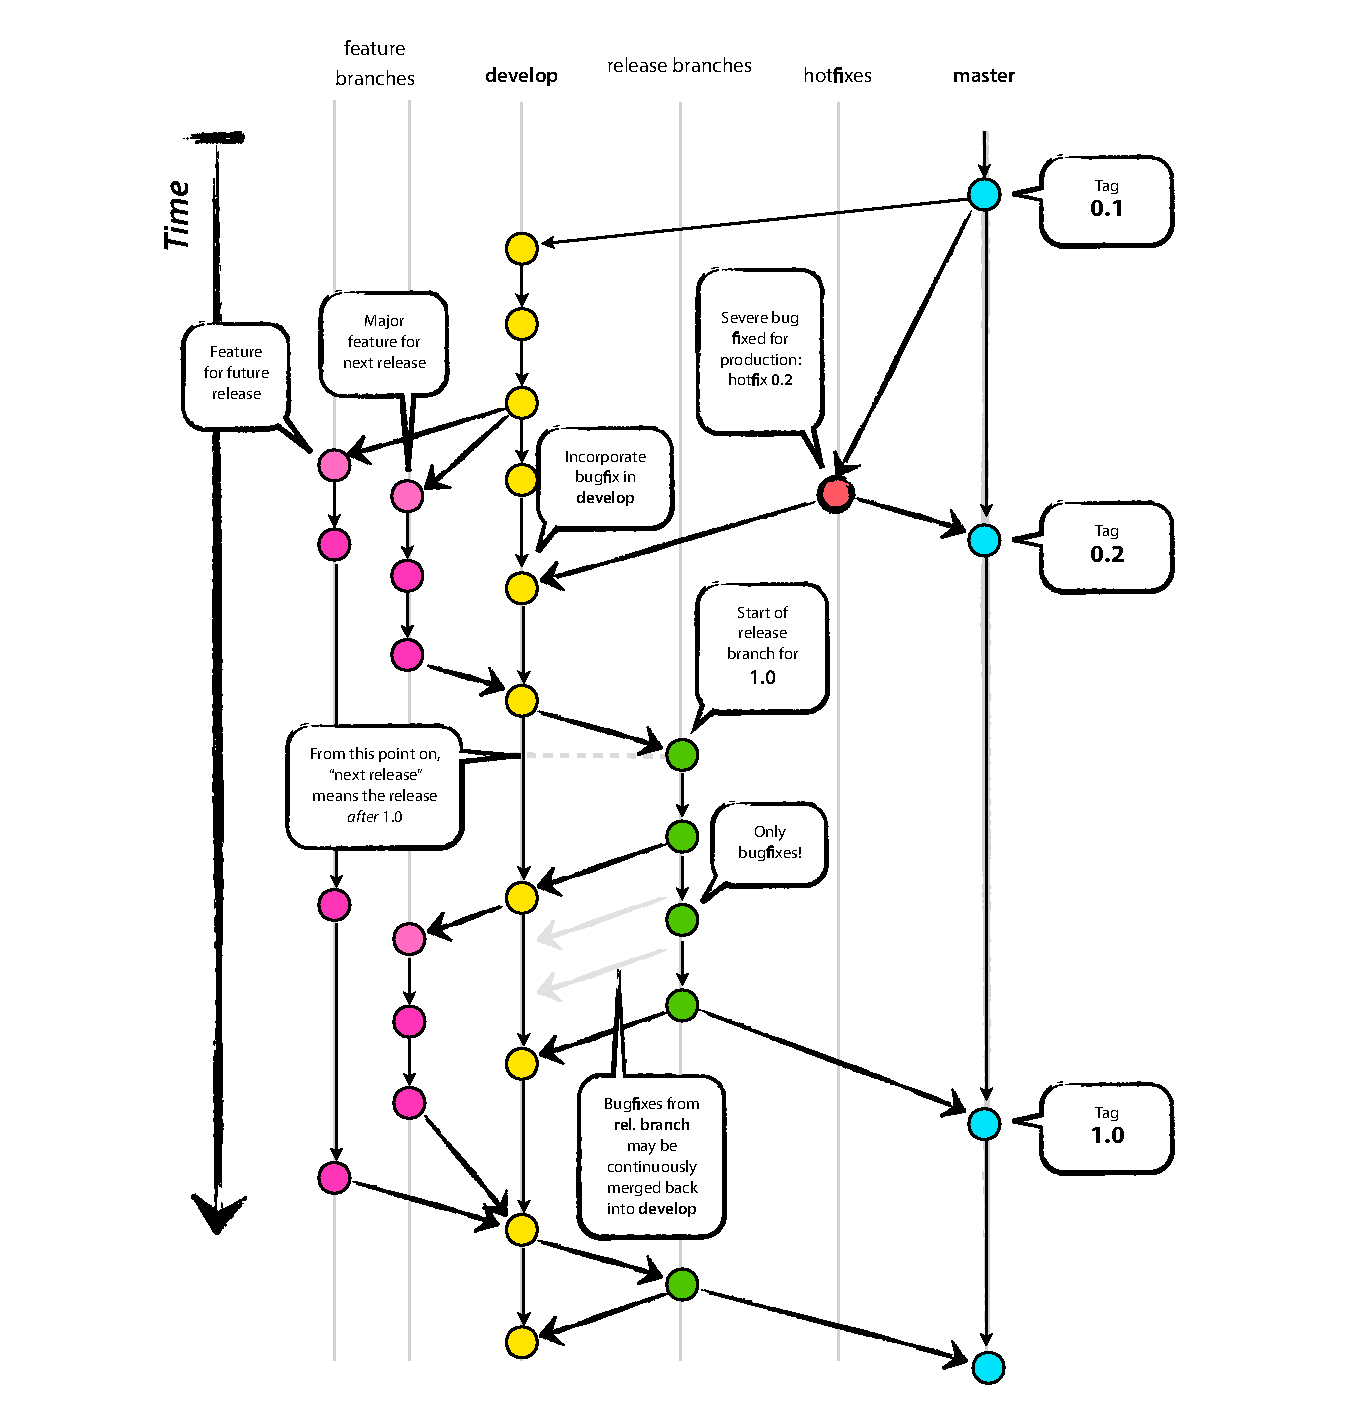
\includegraphics[width=1.0\textwidth]{graphics/gitflow-model.pdf}
	% \caption{\footnotemark[2]}
	\caption[Caption for LOF]{git workflow\protect\footnotemark[1]}
	\label{fig:gitflow}
\end{figure}
\fancyfootnotetext{1}{原作者:Vincent Driessen 地址:http://nvie.com/posts/a-successful-git-branching-model/ 本文稍作修改。}

\subsection{开发规范}
\par 以前端开发规范为例:
\begin{enumerate}[label=(\arabic*)]
    \item 代码规范,\urlstyle{sf} \url{http://google-styleguide.googlecode.com/svn/trunk/};
    \item 目录结构,js、images、css(less/sass),test目录文件结构;
    \item js库依赖,bower;
    \item 使用sass,less、coffeescript,jade等需要编译的文件,即时编译;
    \item UI库(sprites、js的类,常见的,popup,tab,slider,tip等等);
    \item 版本管理,git;
    \item js、css压缩合并,grunt,gulp等;
    \item wiki: MediaWiki;  
    \item bug管理: bugzilla;    
    \item 防止缓存:grunt;
    \item Unit test,e2e测试,集成测试;      
    \item 安全,最常见的是XSS和CSRF。
\end{enumerate}

\fancyfootnotetext{1}{本文源代码地址:}